\begin{figure}[htbp]
    \centering
    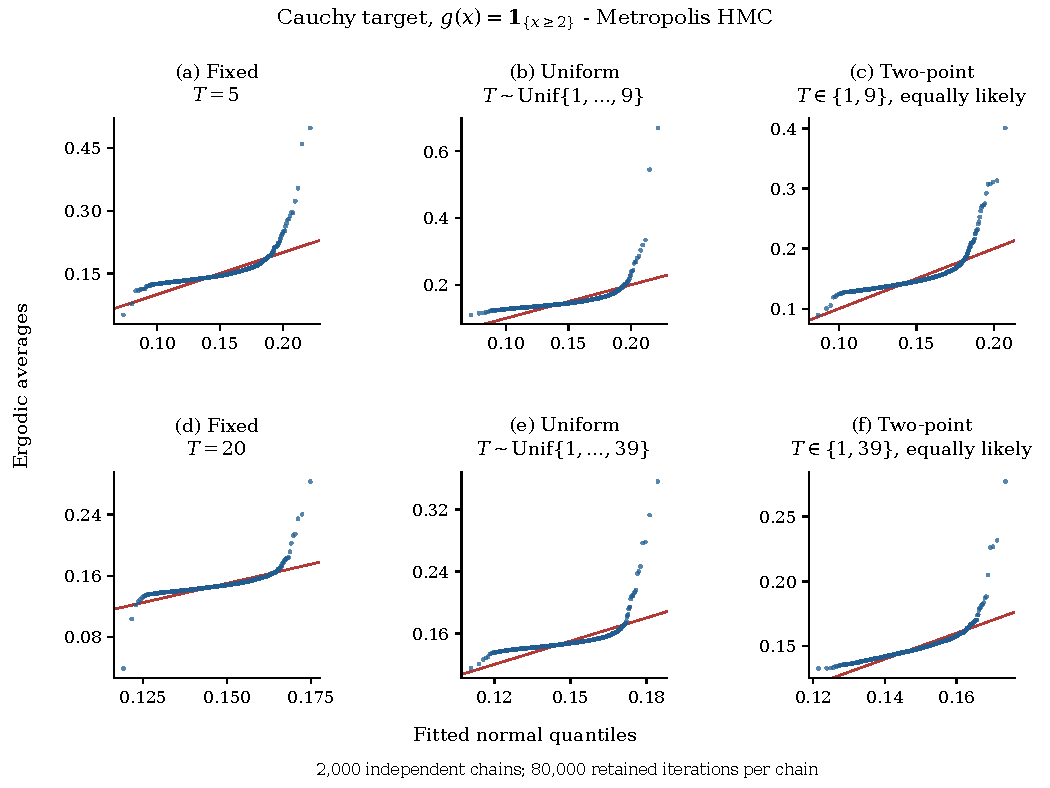
\includegraphics[width=\textwidth]{figures/02_randomisation_and_length.pdf}
    \caption{Trajectory length and independent randomisation for
    Metropolis-adjusted HMC. Here the target is standard Cauchy,
    $U(x)=\log(1+x^2)$, and the observable is
    $g(x)=\mathbf{1}_{\{x\geq2\}}$.
    Rows have mean leapfrog count $m=5$ and $m=20$.
    Columns use $T=m$, $T\sim\mathrm{Unif}\{1,\ldots,2m-1\}$, and
    $T\in\{1,2m-1\}$ with equal probabilities, respectively; random counts
    are redrawn independently at each iteration. Expected leapfrog work is
    equal within each row, while $\mathbb{E}[T^2]$ differs.
    Each panel uses 2,000 independent chains and 80,000 retained observations
    per chain. Initialisation, burn-in, step size, unit mass and the raw
    Gaussian QQ construction are as in
    Figure~\ref{fig:ula-fixed-random}. These are finite-run distributional
    comparisons.}
    \label{fig:randomisation-length}
\end{figure}
